% !TEX encoding = IsoLatin
%
% 1. process this file with pdflatex
% 2. remind to process it twice otherwise cross-references will be wrong
%
\documentclass[a4paper,12pt]{article}
%
% This is to create hyperlinks for index, URLs and citations
% (now we can use the command \url{...} to create URL with hyperlink)
% 
\usepackage{color}
\usepackage[a4paper,colorlinks=true,urlcolor=blue,citecolor=blue,linkcolor=blue,bookmarks=false]{hyperref}
%
% This allows inclusion of pictures.
% Create figures with PowerPoint and then export them individually
% in PDF, PNG, JPEG, or GIF format (in order of preference)
%
\usepackage[pdftex]{graphicx}
\DeclareGraphicsExtensions{.pdf,.png,.jpg,.gif}
%
% phantom space (for abbreviations)
%
\usepackage{xspace}
%
% to insert a proper DOI (Digital Object Identifier)
%
\usepackage{doi}
\renewcommand{\doitext}{DOI }
%
% Definition of margins
%
\usepackage[top=2cm,bottom=2cm,left=2cm,right=2cm]{geometry}
%
% to specify international measure units (also binary ones)
\usepackage[binary-units]{siunitx}
% use / rather than power -1 for "per second" units
\sisetup{per-mode=symbol}
%
% per inserire codice di programmazione complesso
\usepackage{listings}% per inserire codice di programmazione complesso
\lstset{
basicstyle=\ttfamily,
columns=fullflexible,
xleftmargin=3ex,
breaklines,
breakatwhitespace,
escapechar=`
}
%
% definition of language, change according to the language used
%
\usepackage[english]{babel}
%\usepackage[italian]{babel}
%
% This is needed if you write the report in Italian
%
\usepackage[latin1]{inputenc}% IMPORTANT! use ISO-8859-1 encoding
%
% Paragraph skip and indent
%
\setlength\parskip{\medskipamount}
\setlength\parindent{0pt}
%
% Frequently used abbreviations.
% - example1: \ie this is an example
% - example2: the \ipsec protocol
% You can define additional ones.
%
\def\eg{e.g.\xspace}
\def\ie{i.e.\xspace}
\def\ipsec{IPsec\xspace}
\def\myfig#1{Fig.~#1\xspace}
\def\mytab#1{Tab.~#1\xspace}
\def\rfc#1{RFC-#1\xspace}% usage: \rfc{1422}
% to insert a short command-line example
\newcommand{\cmd}[1]{\texttt{#1}\xspace}
%
\begin{document}

\title{Security analysis of the XYZ protocol
\\
{\normalsize Report for the Computer Security exam at the Politecnico di Torino}
}
\author{Giovanni Pautasso (31415)
\\
{\normalsize tutor: Jack-The-Ripper}
}
\date{September 2018}
\maketitle

\vfill

\rule{\textwidth}{1pt}

\tableofcontents

\rule{\textwidth}{1pt}

\vfill

\newpage

\section{Introduction}

Explain here why the XYZ protocol is important
and what was the purpose of the present work.

If you want to reference a web site you can do in-line like this --
\url{http://www.polito.it} -- or you can put it in the bibliography when it refers to a project, such as the OpenSSL one \cite{openssl}.

\begin{figure}[tb]
\begin{lstlisting}
#include <stdio.h>

int main ()
{
   printf ("Hello!\n");
   return 0;
}
\end{lstlisting}
\caption{An example of a program inserted via \cmd{lstlisting}.\label{fig:prog}}
\end{figure}
If you want to display source code or program output, you can use the \cmd{lstlisting} environment which includes text without altering the original formatting and uses a fixed space font, as in the example in Fig.~\ref{fig:prog}.
You can also give numbers to the lines of the program, as in the example in Fig.~\ref{fig:prog-num}, but numbering should be used only if the text explicitly references  specific sections of the  program.

\begin{figure}[tb]
\begin{lstlisting}[numbers=left]
#include <stdio.h>

int main ()
{
   printf ("Hello!\n");
   return 0;
}
\end{lstlisting}
\caption{Example of a program inserted via \cmd{lstlisting} with line numbering.\label{fig:prog-num}}
\end{figure}

To cite short pieces of code you can use directly \cmd{lstlisting} in the body text (rather than in a separate figure), as in the following example related to the HTML code for centering a text:
\begin{lstlisting}
<center>
Example of centered text.
</center>
\end{lstlisting}


\section{Protocol description}

Describe the protocol in detail, trying to demonstrate knowledge
of the topics covered in the course. In other words, don't limit
yourself just to list security features but explain why they are
important and provide your opinion if they are correctly implemented
or could be improved.

You can reference a figure by using the appropriate command,
as in the case of \myfig{\ref{fig:handshake}},
that will be automatically placed on the page and numbered by LaTeX.
(NOTE: read the comments in the LaTeX source for this figure as it explains the proper scaling of a figure and the three possible ways to insert it).

\begin{figure}
% If the picture uses fonts of the correct size (10 ... 12 pt)
% then it can be included without scaling
\centerline{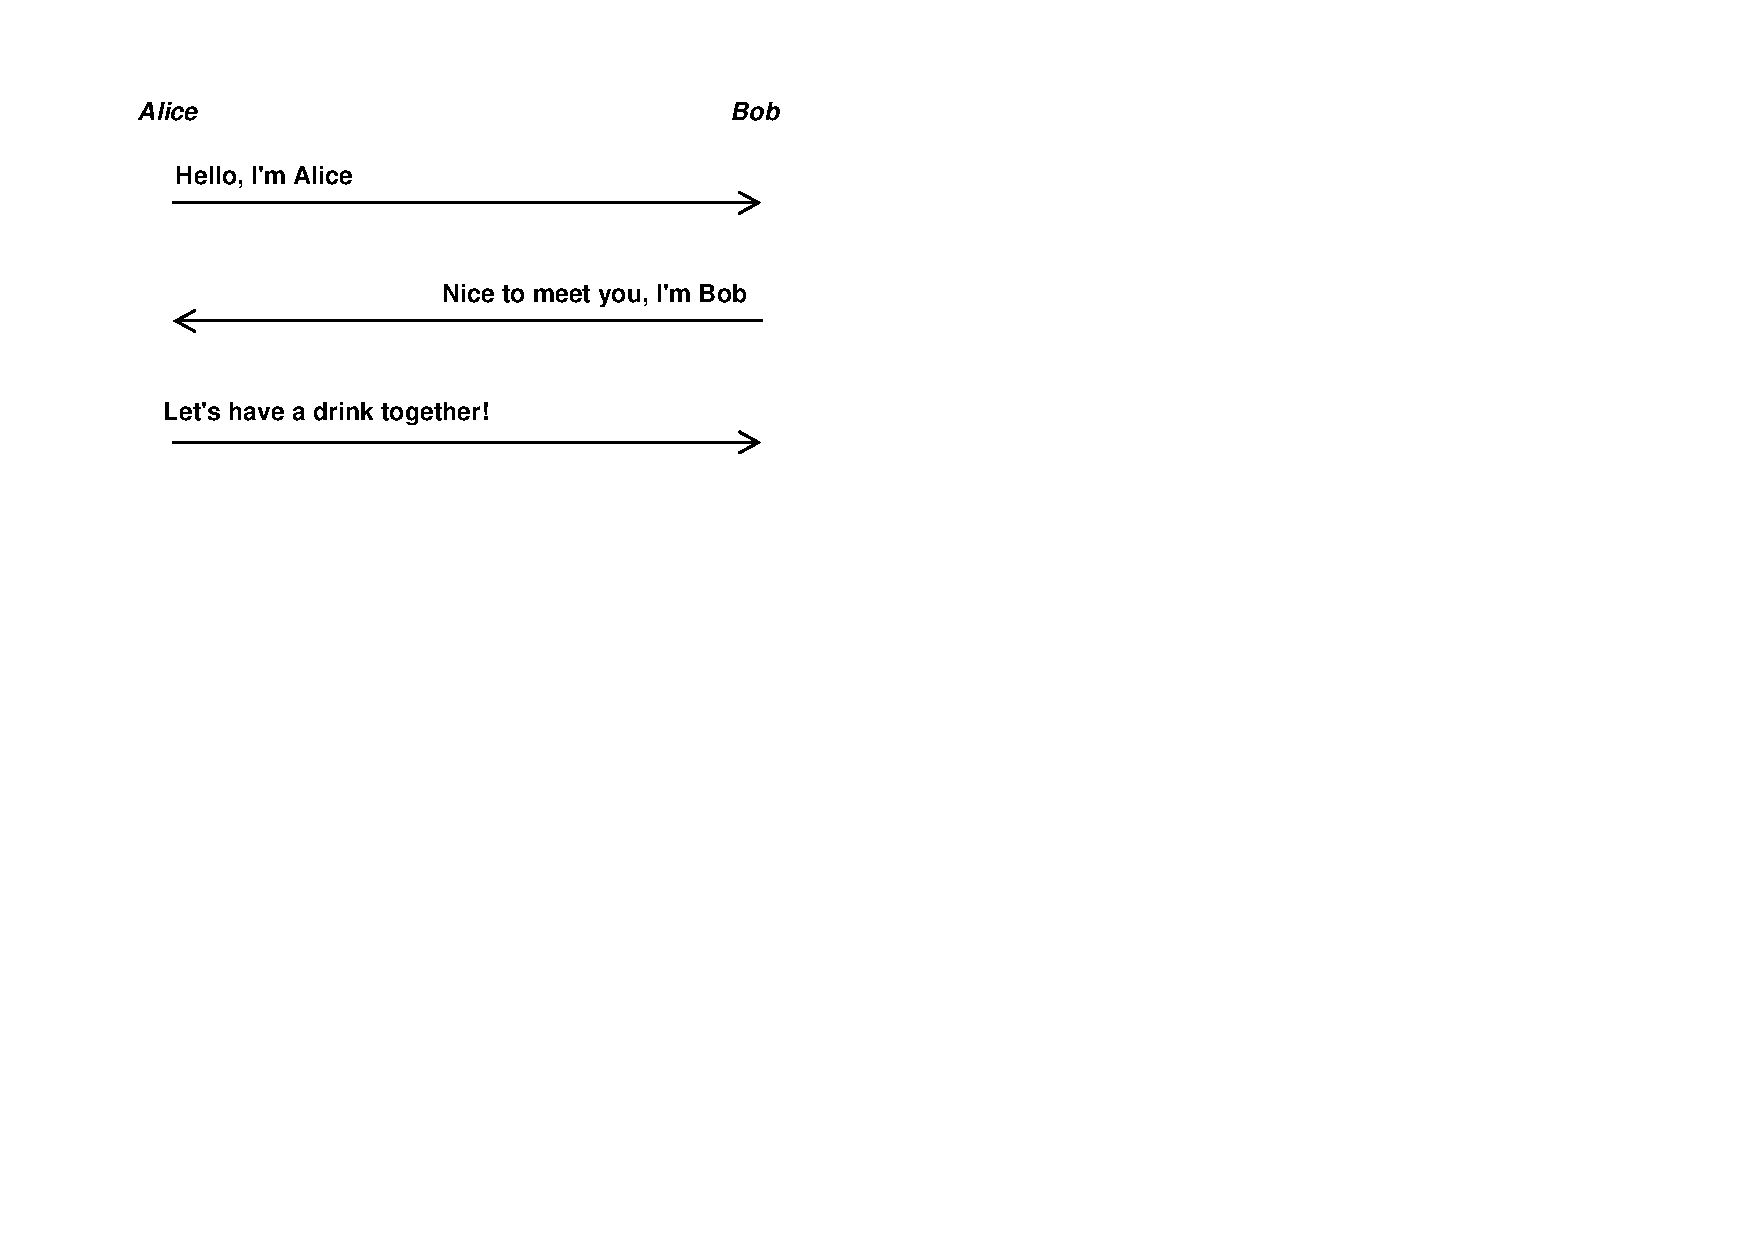
\includegraphics{handshake.pdf}}
% otherwise see the example in the following (commented out) line
% to scale it 50% (e.g. 20pt font get scaled to 10pt font)
%   \centerline{\includegraphics[scale=0.5]
% if you have a picture (i.e. no text hence no font size problem)
% you can fit it relatively to the page width
%   \centerline{\includegraphics[width=0.9\textwidth]
\caption{Handshake protocol.}
\label{fig:handshake}
\end{figure}

You can also cite papers published at conferences, like \cite{psisec}, or journals \cite{tpa}, an RFC \cite{tls12}, a book \cite{seceng}, or a chapter in a multi-author book \cite{tc}.

If the section contains a lot of information, you may want to split it into different subsections, each one with a specific focus as done here.

\subsection{Request format}
The request contains the ID of the caller and the destination IP address, encoded in four different bytes.

On average, it is \SI{10}{\mega\byte} in size. (NOTE: use the siunitx package to properly insert international units when needed, see the LaTeX source for an example on this line and also in Table~\ref{tab:results}).

\subsection{Response format}
The response contains a status code (three digits encoded in ASCII)
followed by the answer encoded in ISO-8859-1 and terminate with CR LF.

\section{Experimental evaluation}
Describe:
\begin{itemize}
\item general purpose of the experiments (functional evaluation,
performance evaluation, comparison with other stuff)
\item experimental setup (hardware and software, including detailed build and configuration instructions if needed)
\end{itemize}
Then describe each experiment: its specific purpose (\eg\ testing a specific feature of the protocol), the command run, and the output (expected and actual).
You can use a table like \mytab{\ref{tab:results}} to group the results (for example if the same experiment was repeated with several data sizes)
\begin{table}
\begin{center}
\begin{tabular}{|c|c|c|} % three centered columns (but you can also use 'r' for right or 'l' for left)
\hline
{\em data size} & {\em raw transfer time} & {\em secure transfer time} \\
(\si{\kilo\byte}) & (\si{\milli\second}) & (\si{\milli\second})\\
\hline
128  & 20  & 22 \\
256  & 22  & 30 \\
512  & 26  & 37 \\
1024 & 30  & 99 \\
\hline
\end{tabular}
\end{center}
\caption{Experimental results.}
\label{tab:results}
\end{table}

For performance testing, remember to run not only experiments with various data size but also -- in case of a client-server protocol -- stress tests for the server (\ie\ increasing number of clients simultaneously requesting attention from the server).
Normally the throughput is measured in \si{\mega bps}.

\section{Style}

Before delivering your report, don't forget to run a spell checker (MikTeX has an embedded one with a UK-English dictionary).

Remember the difference between open and closed quotes in the normal text and note that LaTeX does them by doubling single quotes ``as in this example''.

Use ISO-8859-1 characters (not UTF-8 which is badly supported is some environments).


% if your bibligraphy is trivial then you can insert elements formatting them by yourself according to this example
%% !TEX encoding = IsoLatin

% La bibliografia, da inserirsi solo se ci sono state citazioni.
% In questo caso ricordarsi che bisogna sempre elaborare due volte il file .TEX
% perch� la prima volta viene generata la bibliografia mentre la seconda volta viene inclusa

% NOTA: citare il DOI non � obbligatorio ma MOLTO desiderabile
% NOTE: inserting the DOI is not compulsory bur STRONGLY recommended whenever it exists

\begin{thebibliography}{9} % se ci sono meno di 10 citazioni
%\begin{thebibliography}{99} % se ci sono da 10 a 99 citazioni
%\begin{thebibliography}{999} % se ci sono da 100 a 999 citazioni

% esempio citazione articolo a congresso
% example: reference to a conference paper
\bibitem{psisec}
% autori - authors
I.Enrici, M.Ancilli, A.Lioy,
% titolo articolo - article title
``A psychological approach to information technology security'',
% nome del congresso - conference name
HSI-2010: 3rd Int. Conf. on Human System Interactions,
% luogo (stato) e data del congresso
% town (country) and date of the conference
Rzesz�w (Poland), May 13-15, 2010,
% pagine dell'articolo - article pages
pp.\ 459-466,
% DOI
\doi{10.1109/HSI.2010.5514528}

% esempio citazione articolo su rivista
% example: reference to a journal/magazine article
\bibitem{tpa}
% autori- authors
G.Cabiddu, E.Cesena, R.Sassu, D.Vernizzi, G.Ramunno, A.Lioy,
% titolo dell'articolo -  article title
``Trusted Platform Agent'',
% nome della rivista - name of the journal
IEEE Software,
% volume e numero della rivista (alcune riviste non ce l'hanno)
% volume and issue number (some journals don't have it)
Vol.\ 28, No.\ 2,
% mese e anno di pubblicazione della rivista
% month and year when paper appeared in the journal
March-April 2011,
% pagine dell'articolo  - article pages
pp.\ 35-41,
% DOI
\doi{10.1109/MS.2010.160}


% esempio citazione capitolo di un libro fatto come collezione di contributi da autori diversi
% example: reference to the chapter of a book which is a collection of chapters from different authors
\bibitem{tc}
A.Lioy, G.Ramunno, % autori del capitolo
``Trusted Computing'' % titolo del capitolo
nel libro % in the book
``Handbook of Information and Communication Security'' % titolo del libro
a cura di % edited by
P.Stavroulakis, M.Stamp, % nomi dei curatori
Springer, % nome editore
2010, % anno di pubblicazione
pp.\ 697-717, % pagine del capitolo
\doi{10.1007/978-3-642-04117-4_32}

% esempio citazione pagina web di un progetto
% example: reference to the web page pof a project
\bibitem{openssl}
% nome del progetto - name of the project
The OpenSSL project,
 % URI della pagina web - URI of the web page
\url{http://www.openssl.org/}

% esempio citazione RFC
% example: reference to a RFC
\bibitem{tls12}
T.Dierks, E.Rescorla,
``The Transport Layer Security (TLS) Protocol Version 1.2'',
\rfc{5246}, August 2008,
\doi{10.17487/RFC5246}

% esempio: citazione libro
% example: reference to a book
\bibitem{seceng}
Ross J. Anderson,
``Security engineering'',
Wiley, 2008,
ISBN: 978-0-470-06852-6

\end{thebibliography}


% if your bibliography has been written with Bibtex
\bibliographystyle{torsec}
\bibliography{biblio}


\end{document}

